% --- Aufgabenblatt: Satz des Pythagoras ---

\section*{Aufgabenblatt: Satz des Pythagoras}

\subsection*{1. Grundlagen}
\textbf{a)} Erkläre den Satz des Pythagoras in eigenen Worten.

\textbf{b)} Formuliere die Gleichung für ein rechtwinkliges Dreieck mit den Katheten $a$, $b$ und der Hypotenuse $c$.

\subsection*{2. Einfache Anwendungsaufgaben}
\textbf{a)} Berechne die Hypotenuse $c$ im rechtwinkligen Dreieck mit $a = 3$ cm und $b = 4$ cm.

\begin{center}
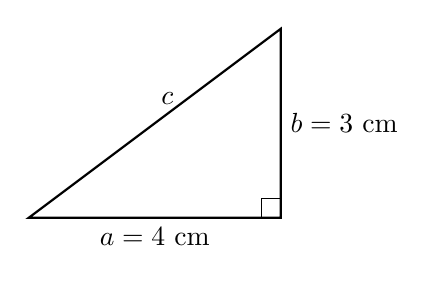
\begin{tikzpicture}[scale=0.8]
  \draw[thick] (0,0) -- (4,0) -- (4,3) -- cycle;
  \draw (2,0) node[below]{$a=4$ cm};
  \draw (4,1.5) node[right]{$b=3$ cm};
  \draw (2.2,1.2) node[above, yshift=10pt]{$c$};
  \draw (4,0) rectangle (3.7,0.3);
\end{tikzpicture}
\end{center}

\textbf{b)} Ein rechtwinkliges Dreieck hat die Katheten $a = 5$ cm und $b = 12$ cm. Berechne $c$.

\vspace{0.5cm}

\subsection*{3. Kathete berechnen}
\textbf{a)} In einem rechtwinkligen Dreieck ist $c = 13$ cm und $a = 5$ cm. Berechne $b$.

\textbf{b)} In einem rechtwinkligen Dreieck ist $c = 10$ cm und $b = 6$ cm. Berechne $a$.

\vspace{0.5cm}

\subsection*{4. Anwendungsaufgaben mit Skizze}
\textbf{a)} Eine Leiter ist 5 m lang und lehnt an einer Wand. Der Fuß der Leiter steht 1,2 m von der Wand entfernt. Wie hoch reicht die Leiter an der Wand? (Skizze)

\begin{center}
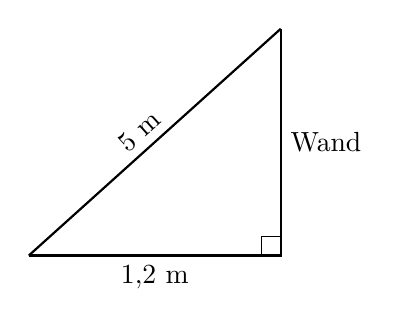
\begin{tikzpicture}[scale=0.8]
  \draw[thick] (0,0) -- (4,0) -- (4,3.6);
  \draw[thick] (0,0) -- (4,3.6);
  \draw (2,0) node[below]{$1{,}2$ m};
  \draw (4,1.8) node[right]{Wand};
  \draw (2.2,1.8) node[above, rotate=42, xshift=-5pt, yshift=3pt]{$5$ m};
  \draw (4,0) rectangle (3.7,0.3);
\end{tikzpicture}
\end{center}

\textbf{b)} Ein Baum wirft einen 8 m langen Schatten. Der Abstand von der Baumspitze zum Ende des Schattens beträgt 10 m. Wie hoch ist der Baum?

\vspace{0.5cm}

\subsection*{5. Anspruchsvollere Aufgaben}
\textbf{a)} Ein Rechteck hat die Seitenlängen 6 cm und 8 cm. Berechne die Länge der Diagonale.

\textbf{b)} In einem gleichschenkligen rechtwinkligen Dreieck ist die Hypotenuse 10 cm lang. Wie lang sind die Katheten?

\textbf{c)} Ein Dreieck hat die Seiten $a = 7$ cm, $b = 24$ cm und $c = 25$ cm. Überprüfe, ob das Dreieck rechtwinklig ist.

\vspace{0.5cm}

\subsection*{6. Knobelaufgabe}
\textbf{a)} Ein Quadrat hat eine Fläche von 50 cm$^2$. Wie lang ist die Diagonale? (Gib das Ergebnis als Wurzel und gerundet an.)

\textbf{b)} Ein rechtwinkliges Dreieck hat ganzzahlige Seitenlängen. Finde drei verschiedene Beispiele (Pythagoreische Tripel).

% --- Ende des Aufgabenblatts ---
